%part2a.tex
\subsection*{a. Stability of the solutions of an ODE-system of LCC-type}
The purpose of this section is to investigate the stability of an ODE while a parameter changes continuously.

The given third-order equation is the following : 
\begin{eqnarray*}
y'''+3y''+2y'+Ky =& 0 \\
y(0) =& 1\\
y'(0)=&1\\
y''(0)=&1
\end{eqnarray*}

It is possible to rewrite this as a system of ODE's, introducing new variables.
\begin{eqnarray*}
\textbf{u'}  = \left( \begin{array}{c}
y' \\ 
y'' \\ 
y'''
\end{array} \right) =& \left( \begin{array}{ccc}
0 & 1 & 0 \\ 
0 & 0 & 1 \\ 
-K & -2 & -3
\end{array}  \right) \left( \begin{array}{c}
y \\ 
y'\\ 
y''
\end{array} \right) = \textbf{Au} 
\end{eqnarray*}
The initial conditions are rewritten by :
\begin{eqnarray*}
\textbf{u(0)} =& \left( \begin{array}{c}
y(0) \\ 
y'(0)\\ 
y''(0)
\end{array} \right) = \left( \begin{array}{c}
1\\ 
1\\ 
1
\end{array} \right) 
\end{eqnarray*}

The solutions, computed analytically for different values of K, are given in figure \ref{result21}. The Matlab code is given at the end of this section. It is possbile to see that for the first three values of K, the maximal amplitude of the blue curve (that is the function $y$) tends to decrease. This being an LCC system, we know that a perturbation will follow the same ODE so we can conclude that the system is stable for those values of K. On the other hand, for the last value ($K=8$), this amplitude increases. Hence, the system is not stable for $K=8$. By continuity, that means that the system becomes unstable for a value of K between $4$ and $8$. Because we know nothing else, the best estimation that we can give right now is that this value is $K=6$.\\

\begin{figure}
\begin{center}
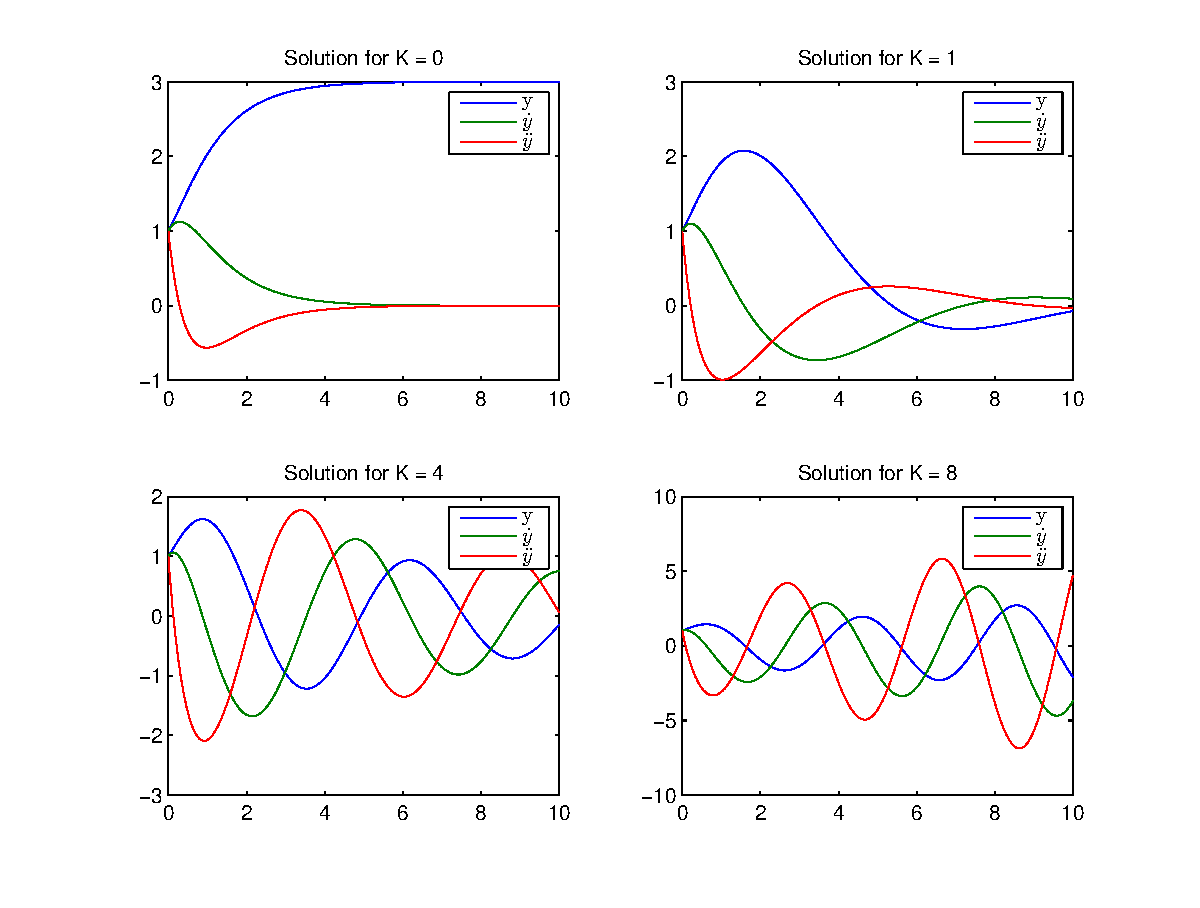
\includegraphics[scale=0.5]{result21.eps}
\caption{Solutions of the system in part 2a for various values of K}
\label{result21}
\end{center}
\end{figure}

We then drew a root locus to see how the system would evolve if K varies continuously. Again, the code is given at the end of the section. We used the built-in function $rlocus$. In order to do so, we first have to compute the transfert function of the process that is equivalent to our differential equation with an unit feedback with gain K. One can show that this transfert function $H(s)$ is :
$$H(s) = \frac{1}{s^3+3s^2+2s}$$

The figure \ref{rloc} shows the rootlocus. The values of k were chosen so that the curve would be smooth. We can see that as K increases, one eigenvalue is getting more and more negative while the two others first are getting closer then leave the real axis. We can also see that at some point, those two eigenvalues cross the imaginary axis thus making the system unstable.

The next step was to compute the first value of K making the system unstable. It is possible to check each time we increase K if the eigenvalue have a positive real part but the result is only an approximation. It is also possible to compute this value analytically and that is what we did. By continuity, we know that for this value, two eigenvalues are located on the imaginary axis so :
$$\lambda = xj$$
With $x$ a real number. We then plug that into the caracteristic equation.
\begin{eqnarray*}
\lambda ^3+3\lambda ^2+2\lambda +K=&0\\
-x^3j-3x^2+2xj+K=&0\\
\left(\begin{array}{c}
K-3x^2 \\ 
2x-x^3
\end{array} \right) =& \left( \begin{array}{c}
0 \\ 
0
\end{array} \right)
\end{eqnarray*}

We have the trivial solution ($x=K=0$) but we are not interested in that one. The two others are :
\begin{eqnarray*}
x =& \pm \sqrt{2}\\
K =& 6
\end{eqnarray*}

So we can conclude that :
$$\textit{The system is unstable} \iff K>6$$

\begin{figure}
\begin{center}
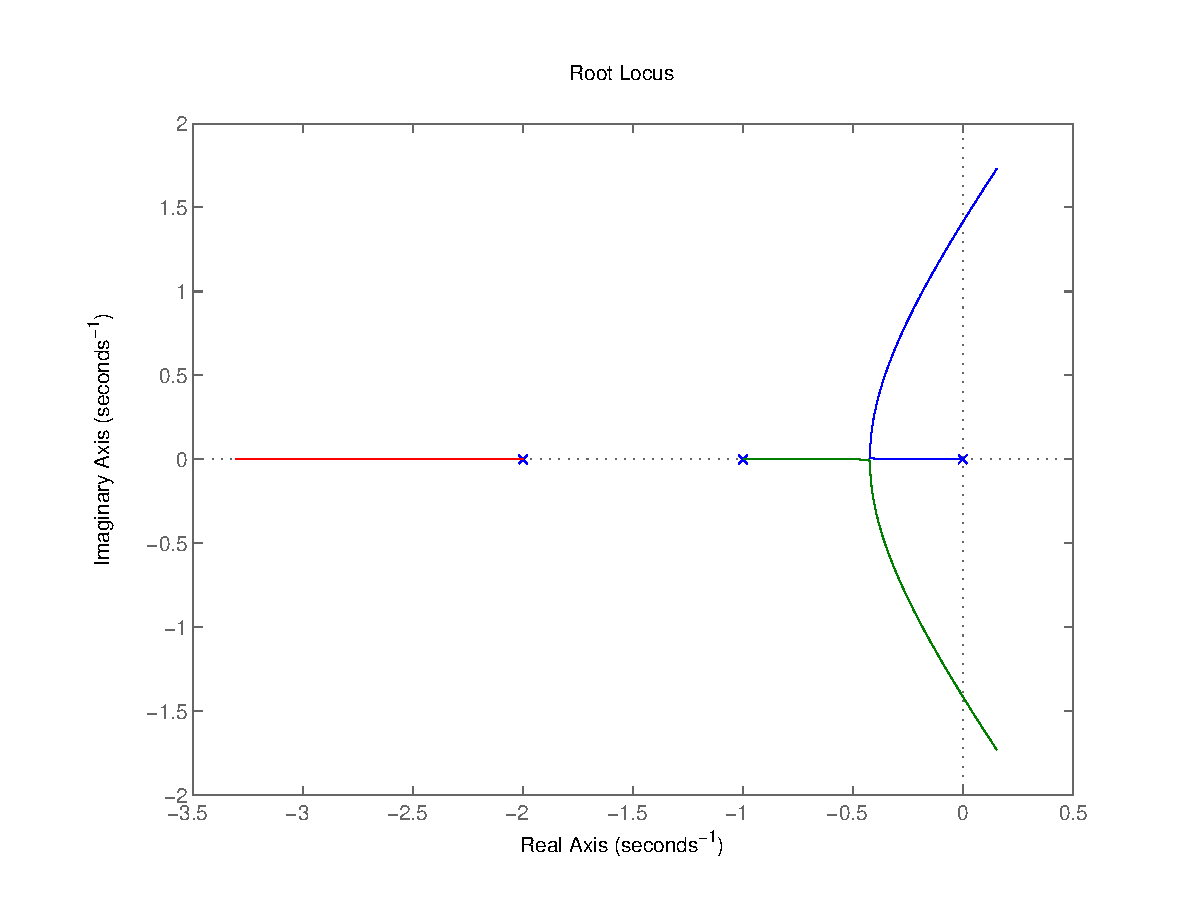
\includegraphics[scale=0.5]{rloc.eps}
\caption{Root locus of $y'''+3y''+2y'+Ky=0$}
\label{rloc}
\end{center}
\end{figure}


%Ce truc insere mon code MATLAB (nice!) 
\lstinputlisting{LAB1_21.m}